\setlength{\columnsep}{3ex}
\begin{wrapfigure}[27]{r}{.4\textwidth}
\centering
\vspace*{-5ex}
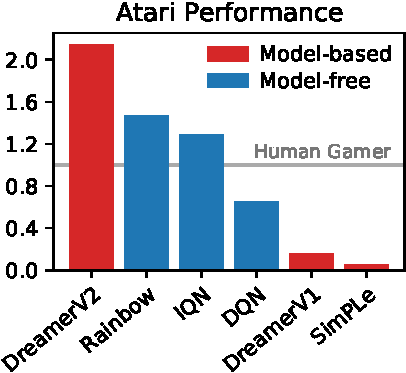
\includegraphics[width=\linewidth]{first/first}
\vspace*{-3.3ex}
\caption{Gamer normalized median score on the Atari benchmark of 55 games with sticky actions at 200M steps.
DreamerV2 is the first agent that learns purely within a world model to achieve human-level Atari performance, demonstrating the high accuracy of its learned world model. DreamerV2 further outperforms the top single-GPU agents Rainbow and IQN, whose scores are provided by Dopamine \citep{castro2018dopamine}.
According to its authors, SimPLe \citep{kaiser2019simple} was only evaluated on an easier subset of 36 games and trained for fewer steps and additional training does not further increase its performance.}
\label{fig:first}
\end{wrapfigure}

% \setlength{\columnsep}{3ex}
% \begin{wrapfigure}[22]{r}{.39\textwidth}
% \centering
% \vspace*{-4.5ex}  % -2.1ex
% 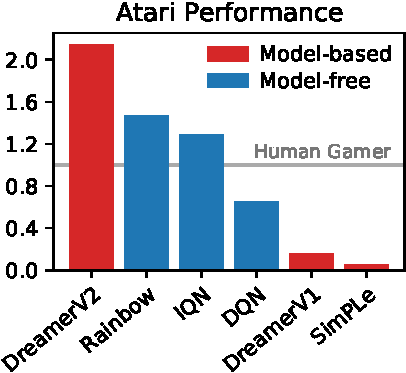
\includegraphics[width=\linewidth]{first/first}
% \vspace*{-3.3ex}
% \caption{Gamer normalized task median score on the Atari benchmark of 55 games with sticky actions at 200M frames. DreamerV2 substantially improves over previous model-based agents, outperforming both human gamer and top-model free agents.}
% \label{fig:first}
% \end{wrapfigure}
% \footnotetext{According to its authors, SimPLe \citep{kaiser2019simple} was only evaluated on an easier subset of 36 games and trained for fewer steps and additional training does not further increase its performance. We computed its median score from Table 3 in their paper.}